\documentclass[10pt, a4paper]{article}
\usepackage{amsmath}
\usepackage{amssymb}
\usepackage{mathtools}
\usepackage{mathtext}
\usepackage[T1, T2A]{fontenc}
\usepackage[utf8]{inputenc}
\usepackage[english, russian]{babel}
\usepackage{cmap}
\usepackage{fancyhdr}
\usepackage[pdftex]{graphicx}
\usepackage{gensymb}
\usepackage{floatrow}
\usepackage{titlesec}
\usepackage{lastpage}
\usepackage{float}
\usepackage{gensymb}
\usepackage{booktabs}
\usepackage{mathrsfs}
\usepackage{floatflt}
\usepackage{wrapfig}
\usepackage{caption}

\begin{document}
\begin{titlepage}
    \centering
    
    \vfill
    
    \vfill
    {\huge\bfseries
   Промпт-атаки на большие языковые модели (LLM) 
    }
    \vfill
  
    
  
    \vfill
  
    Юшин С.В.
  \end{titlepage}
  \newpage

  \section{Задача}
  #1.Вникнуть в тематику, разобраться с тем чем GenAI (в частности LLM) отличается от классических алгоритмов AI. Разобраться в уязвимостях специфичных для GenAI, как на этапе обучения, так и на этапе эксплуатации модели.

2.Подготовить список актуальных промпт-атак, реализуемых через окно диалога.  Отдельное внимание уделить промпт-атакам в части кибербезопасности (КБ). «Использование LLM модели как инструмента подготовки кибератаки» - генерация вредоносного кода, социальная инженерия, фишинг и т.п. Поискать в открытых источниках и научных публикациях.

3.Попробовать провести промпт-атаку на LLM модели в свободном доступе. Оценить успешность атаки.

  \section{Оборудование}
  В работе используется: оптическая скамья, осветитель, два длиннофокусных объектива кювета с жидкостью, кварцевый излучатель с микрометрическим винтом, генератор У.З. волны, линза, вертикальная нить на рейтере, микроскоп.

  \section{Теоретические сведения}
Источник света Л с помощью конденсора К проецируется на входную (коллиматорную) щель S. Входная щель ориентирована горизонтально и прикрыта красным светофильтром Ф. Коллиматорный объектив $ О_1 $ посылает параллельный пучок на кювету с водой C. Излучатель Q, погружённый в кювету, создаёт УЗ-волну. Вертикальное перемещение излучателя осуществляется винтом I, тонкая подача — лимбом II. При определённых положениях излучателя волна становится стоячей.

\begin{figure}[H]
	\centering
	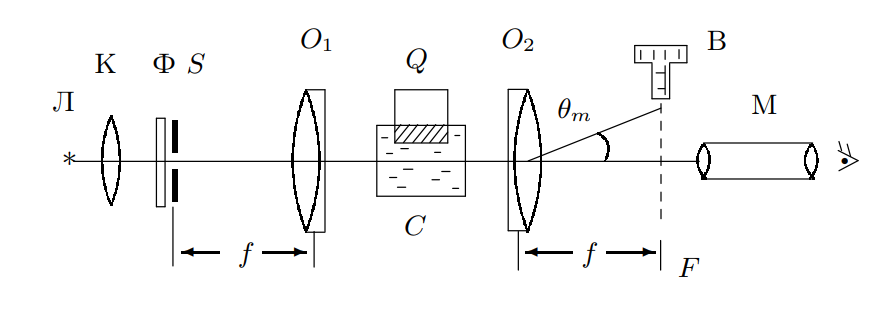
\includegraphics[width=1\linewidth]{Screenshot_1}
	\caption{Схема экспериментальной установки}
	\label{fig:screenshot1}
\end{figure}
Пусть фаза световых колебаний на передней поверхности жидкости равна нулю. Тогда на задней поверхности (т.е. в плоскости $ z=0 $) она равна \[\varphi = k n L = \varphi_0(1+m \cos \Omega x),\]
где $ L $ -- толщина слоя жидкости в кювете, $ k = 2 \pi /\lambda $ -- волновое число для света, $\lambda $ -- длина световой волны, $ \varphi_0 = k n_0 L $. Таким образом, в плоскости $ z=0 $ фаза световых колебаний является периодической функцией координаты $ x $, иными словами — УЗ-волна в жидкости создаёт фазовую дифракционную решётку.

Её функция пропускания:
\begin{equation}\label{eq:1}
	t(x) = e^{i m \cos \Omega x} \overset{m \ll 1}{\approx} 1 + \frac{im}{2}e^{i \Omega x} + \frac{im}{2}e^{-i \Omega x}.
\end{equation} 
При освещении этой решётки плоской нормально падающей волной амплитуды $ a $ имеем за решёткой (при $ z > 0 $):
\[f(x, z) = a e^{i k z} + \frac{i a m}{2} e^{i(\Omega x +\sqrt{k^2-\Omega^2 } z )}+\frac{i a m}{2} e^{i(-\Omega x +\sqrt{k^2-\Omega^2 } z )}\]
При изучении дифракции методом тёмного поля будем удалять компоненту $ f_0 = a e^{i k z} $ ставя проволочку в соответствующем месте фурье-плоскости. В этом состоит метод тёмного поля в изучении фазово-контрастных объектов. 

При небольших амплитудах звуковой волны показатель преломления жидкости n меняется по закону
\[n=n_0(1+m \cos \Omega x),\]
где $ \Omega $ -- волновое число УЗ волны, $ m\ll 1 $ -- глубина модуляции УЗ волны.

В общем случае после прохождения через кювету световое поле представляет совокупность не трёх, а большого числа плоских волн, распространяющихся под углами, определяемыми условием \begin{equation}\label{eq:лямбдасинустета}
	\Lambda \sin \theta_m = m \lambda, \; m\in \mathbb{Z}.
\end{equation}
Каждая из этих волн соответствует одному из максимумов в дифракционной картине Фраунгофера.
Определяя на опыте положение дифракционных максимумов различного порядка, можно по формуле ()\ref{eq:лямбдасинустета}) найти длину $ \Lambda $ УЗ-волны и вычислить скорость $ v $ распространения ультразвуковых волн в жидкости, если известна частота $ \nu $ колебаний кварцевого излучателя:
\[v = \Lambda \nu .\] 

\section{Результаты измерений и обработка данных}
\paragraph{Исследование по дифракционной картине. }

Оценим \emph{по порядку величины} скорость звука как удвоенное расстояние между наиболее чёткими дифракционными картинами:
\[n = 67 \;дел,\]
\[\lambda \approx 67*10*2=1340 \; мкм. \]
Отсюда 
\[v = \lambda * \nu \approx 1640 \; м/с.\]
Эта величина не является точной, т. к. оценка проводилась по факту наибольшей видимости, поэтому подсчёт погрешностей не имеет смысла.

Определим положения дифракционных полос. Более 5 полос получить не удалось, т. к. генератор имеет низкую чувствительность ручки, а на высоких частотах ($ \gtrsim 5 \; МГц $) выдаёт нестабильную частоту. Результаты в табл. \ref{tab:result}.

% Please add the following required packages to your document preamble:
% \usepackage{multirow}
\begin{table}[h]
	\centering
	\begin{tabular}{|l|l|l|l|l|l|}
		\hline
		\multirow{2}{*}{$\nu, \; МГц$} & \multicolumn{5}{l|}{a, мкм, в порядке n} \\ \cline{2-6} 
		& -2    & -1     & 0      & +1    & +2     \\ \hline
		1.4570                         & -344   & -172  & 0   & 196    & 384 \\ \hline
		2.1515                         & ---    & -260  & 0  & 272    & ---  \\ \hline
		4.3971                         & ---    & -540  & 0   & 584    & --- \\ \hline
	\end{tabular}
	\caption{Результаты измерений}
	\label{tab:result}
\end{table}

\begin{figure}[tbp]
	\centering
	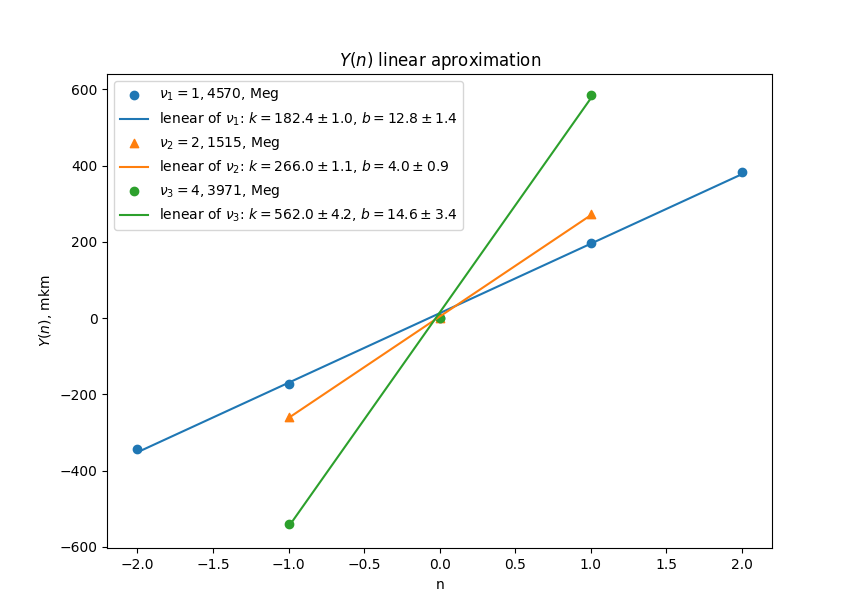
\includegraphics[width=0.8\linewidth]{Figure_1.png}
	\caption{Графики зависимости $Y = Y(n)$
      $(Y - мкм, n - б/р)$}
	\label{fig:2}
\end{figure}


По результатам получим график на рис. \ref{fig:2}. В табл. \ref{tab:2} коэффициенты прямых и полученные по ним результаты из формулы \begin{equation}\label{eq:2}
	v =\nu m f \lambda / l_m = \nu f \lambda / k .
\end{equation} 


\begin{table}[H]
	\centering
	\begin{tabular}{|l|l|l|l|}
		\hline
		$\nu, \; МГц$ & 1.4570       & 2.1515       & 4.3971       \\ \hline
		$k$           & $182\pm 1$   & $266\pm 1$   & $562\pm 4$  \\ \hline
		$v, \;м/с$    & $1430\pm 20$ & $1450\pm 20$ & $1400\pm 30$ \\ \hline
	\end{tabular}
	\caption{Результат расчёта скорости звука}
	\label{tab:2}
\end{table}

Среднее значение: $$ v = 1430 \pm 50 \; м/с, $$ что близко к табличному значению $ v = 1490  \; м/с $, но не сходится в пределах погрешности. Здесь случайная погрешность среднего взята по формуле среднеквадратичного отклонения (стандартной ошибки) и сложена с инструментальной по формуле $ \sqrt{\sigma^2+\delta^2} $.

\paragraph{Исследование методом тёмного поля. }

Найдём цену деления шкалы микроскопа через период сетки $ h = 1 \;мм $. $ n = 22\; дел/кл $, т. е. $ 1\; дел = 45\; мкм $

По формуле $ \Lambda = 45\;мкм * 2 * n / m $ найдём длину ультразвуковой волны.
Резулаты измерений и расчётов в табл. \ref{tab:3}.

\begin{table}[H]
	\centering
	\begin{tabular}{|l|l|l|l|l|l|l|}
		\hline
		$\nu, \; МГц$     & 1.7070 & 2.0866 & 4.2673 & 2.511 & 3.1819 & 3.8760 \\ \hline
		$n, \; дел$       & 65     & 44     & 43 & 48 & 47 & 30   \\ \hline
		$m, \; линий$     & 8      & 7      & 14 & 9  & 11 & 9 \\ \hline
		$\Lambda, \; мкм$ & 183    & 142    & 69 & 120 & 94 & 75   \\ \hline
	\end{tabular}
	\caption{Результат измерения длин волны}
	\label{tab:3}
\end{table}

\begin{figure}[H]
	\centering
	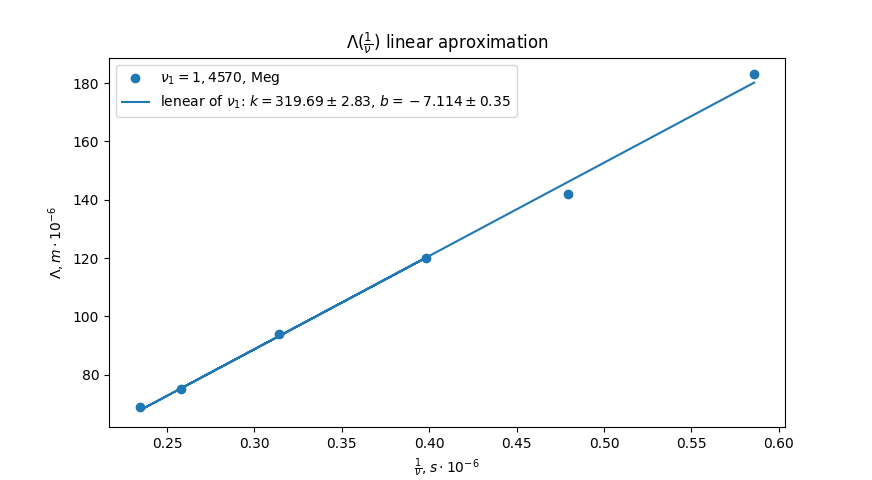
\includegraphics[width=1\linewidth]{Figure_2.png}
	\caption{Зависимость $\Lambda = \Lambda (1/\nu)$}
	\label{fig:3}
\end{figure}


Отсюда по графику на рис. \ref{fig:3} найдём скорость звука в жидкости: 
$$\Lambda = k / \nu + b, k = 319 \pm 3 \; м/с$$
$$ v = 4.5 * k = 1436 \pm 15 \; м/с, $$ 
что согласуется с полученными ранее результатами.

\paragraph{Качественные наблюдения. } Закрывая ненулевые максимумы получаем равномерную засветку, так как интенсивность нулевого максимума многократно превышает интенсивность ненулевых.

\section{Вывод}


Удалось с неплохой точностью измерить скорость звука в воде используя волны сжатие-разряжение как синусоидальную решётку: $v = (1430 \pm 50)\; m/s$, что лежит в пределах двух погрешностей от табличного значения:  $v = 1490\; m/s$\\
Также, была изучена дифракция света на такой акустической решётке;
Был применён и изучен метод тёмного поля в наблюдении фазовых объектов, и найдена с помощбю данного метода скорость звука в воде:$v = (1436 \pm 15)\;m/s$, что хорошо согласуется с экспереминтальным результатом, полученным ранее.


\end{document}